\PassOptionsToPackage{unicode=true}{hyperref} % options for packages loaded elsewhere
\PassOptionsToPackage{hyphens}{url}
%
\documentclass[]{book}
\usepackage{lmodern}
\usepackage{amssymb,amsmath}
\usepackage{ifxetex,ifluatex}
\usepackage{fixltx2e} % provides \textsubscript
\ifnum 0\ifxetex 1\fi\ifluatex 1\fi=0 % if pdftex
  \usepackage[T1]{fontenc}
  \usepackage[utf8]{inputenc}
  \usepackage{textcomp} % provides euro and other symbols
\else % if luatex or xelatex
  \usepackage{unicode-math}
  \defaultfontfeatures{Ligatures=TeX,Scale=MatchLowercase}
\fi
% use upquote if available, for straight quotes in verbatim environments
\IfFileExists{upquote.sty}{\usepackage{upquote}}{}
% use microtype if available
\IfFileExists{microtype.sty}{%
\usepackage[]{microtype}
\UseMicrotypeSet[protrusion]{basicmath} % disable protrusion for tt fonts
}{}
\IfFileExists{parskip.sty}{%
\usepackage{parskip}
}{% else
\setlength{\parindent}{0pt}
\setlength{\parskip}{6pt plus 2pt minus 1pt}
}
\usepackage{hyperref}
\hypersetup{
            pdftitle={P2 - Simulering af Data},
            pdfauthor={Gruppe B2-19},
            pdfborder={0 0 0},
            breaklinks=true}
\urlstyle{same}  % don't use monospace font for urls
\usepackage{color}
\usepackage{fancyvrb}
\newcommand{\VerbBar}{|}
\newcommand{\VERB}{\Verb[commandchars=\\\{\}]}
\DefineVerbatimEnvironment{Highlighting}{Verbatim}{commandchars=\\\{\}}
% Add ',fontsize=\small' for more characters per line
\usepackage{framed}
\definecolor{shadecolor}{RGB}{248,248,248}
\newenvironment{Shaded}{\begin{snugshade}}{\end{snugshade}}
\newcommand{\AlertTok}[1]{\textcolor[rgb]{0.94,0.16,0.16}{#1}}
\newcommand{\AnnotationTok}[1]{\textcolor[rgb]{0.56,0.35,0.01}{\textbf{\textit{#1}}}}
\newcommand{\AttributeTok}[1]{\textcolor[rgb]{0.77,0.63,0.00}{#1}}
\newcommand{\BaseNTok}[1]{\textcolor[rgb]{0.00,0.00,0.81}{#1}}
\newcommand{\BuiltInTok}[1]{#1}
\newcommand{\CharTok}[1]{\textcolor[rgb]{0.31,0.60,0.02}{#1}}
\newcommand{\CommentTok}[1]{\textcolor[rgb]{0.56,0.35,0.01}{\textit{#1}}}
\newcommand{\CommentVarTok}[1]{\textcolor[rgb]{0.56,0.35,0.01}{\textbf{\textit{#1}}}}
\newcommand{\ConstantTok}[1]{\textcolor[rgb]{0.00,0.00,0.00}{#1}}
\newcommand{\ControlFlowTok}[1]{\textcolor[rgb]{0.13,0.29,0.53}{\textbf{#1}}}
\newcommand{\DataTypeTok}[1]{\textcolor[rgb]{0.13,0.29,0.53}{#1}}
\newcommand{\DecValTok}[1]{\textcolor[rgb]{0.00,0.00,0.81}{#1}}
\newcommand{\DocumentationTok}[1]{\textcolor[rgb]{0.56,0.35,0.01}{\textbf{\textit{#1}}}}
\newcommand{\ErrorTok}[1]{\textcolor[rgb]{0.64,0.00,0.00}{\textbf{#1}}}
\newcommand{\ExtensionTok}[1]{#1}
\newcommand{\FloatTok}[1]{\textcolor[rgb]{0.00,0.00,0.81}{#1}}
\newcommand{\FunctionTok}[1]{\textcolor[rgb]{0.00,0.00,0.00}{#1}}
\newcommand{\ImportTok}[1]{#1}
\newcommand{\InformationTok}[1]{\textcolor[rgb]{0.56,0.35,0.01}{\textbf{\textit{#1}}}}
\newcommand{\KeywordTok}[1]{\textcolor[rgb]{0.13,0.29,0.53}{\textbf{#1}}}
\newcommand{\NormalTok}[1]{#1}
\newcommand{\OperatorTok}[1]{\textcolor[rgb]{0.81,0.36,0.00}{\textbf{#1}}}
\newcommand{\OtherTok}[1]{\textcolor[rgb]{0.56,0.35,0.01}{#1}}
\newcommand{\PreprocessorTok}[1]{\textcolor[rgb]{0.56,0.35,0.01}{\textit{#1}}}
\newcommand{\RegionMarkerTok}[1]{#1}
\newcommand{\SpecialCharTok}[1]{\textcolor[rgb]{0.00,0.00,0.00}{#1}}
\newcommand{\SpecialStringTok}[1]{\textcolor[rgb]{0.31,0.60,0.02}{#1}}
\newcommand{\StringTok}[1]{\textcolor[rgb]{0.31,0.60,0.02}{#1}}
\newcommand{\VariableTok}[1]{\textcolor[rgb]{0.00,0.00,0.00}{#1}}
\newcommand{\VerbatimStringTok}[1]{\textcolor[rgb]{0.31,0.60,0.02}{#1}}
\newcommand{\WarningTok}[1]{\textcolor[rgb]{0.56,0.35,0.01}{\textbf{\textit{#1}}}}
\usepackage{longtable,booktabs}
% Fix footnotes in tables (requires footnote package)
\IfFileExists{footnote.sty}{\usepackage{footnote}\makesavenoteenv{longtable}}{}
\usepackage{graphicx,grffile}
\makeatletter
\def\maxwidth{\ifdim\Gin@nat@width>\linewidth\linewidth\else\Gin@nat@width\fi}
\def\maxheight{\ifdim\Gin@nat@height>\textheight\textheight\else\Gin@nat@height\fi}
\makeatother
% Scale images if necessary, so that they will not overflow the page
% margins by default, and it is still possible to overwrite the defaults
% using explicit options in \includegraphics[width, height, ...]{}
\setkeys{Gin}{width=\maxwidth,height=\maxheight,keepaspectratio}
\setlength{\emergencystretch}{3em}  % prevent overfull lines
\providecommand{\tightlist}{%
  \setlength{\itemsep}{0pt}\setlength{\parskip}{0pt}}
\setcounter{secnumdepth}{5}
% Redefines (sub)paragraphs to behave more like sections
\ifx\paragraph\undefined\else
\let\oldparagraph\paragraph
\renewcommand{\paragraph}[1]{\oldparagraph{#1}\mbox{}}
\fi
\ifx\subparagraph\undefined\else
\let\oldsubparagraph\subparagraph
\renewcommand{\subparagraph}[1]{\oldsubparagraph{#1}\mbox{}}
\fi

% set default figure placement to htbp
\makeatletter
\def\fps@figure{htbp}
\makeatother

\usepackage{booktabs}
\usepackage{amsthm}
\makeatletter
\def\thm@space@setup{%
  \thm@preskip=8pt plus 2pt minus 4pt
  \thm@postskip=\thm@preskip
}
\makeatother
\usepackage[]{natbib}
\bibliographystyle{apalike}

\title{P2 - Simulering af Data}
\author{Gruppe B2-19}
\date{2020-02-28}

\usepackage{amsthm}
\newtheorem{theorem}{Sætning}[chapter]
\newtheorem{lemma}{Lemma}[chapter]
\newtheorem{corollary}{Korrolar}[chapter]
\newtheorem{proposition}{Proposition}[chapter]
\newtheorem{conjecture}{Konjektur}[chapter]
\theoremstyle{definition}
\newtheorem{definition}{Definition}[chapter]
\theoremstyle{definition}
\newtheorem{example}{Eksempel}[chapter]
\theoremstyle{definition}
\newtheorem{exercise}{Øvelse}[chapter]
\theoremstyle{remark}
\newtheorem*{remark}{Bemærkning}
\newtheorem*{solution}{Løsning}
\let\BeginKnitrBlock\begin \let\EndKnitrBlock\end
\begin{document}
\maketitle

{
\setcounter{tocdepth}{1}
\tableofcontents
}
\hypertarget{introduktion}{%
\chapter{Introduktion}\label{introduktion}}

\hypertarget{variabeltyper}{%
\chapter{Variabeltyper}\label{variabeltyper}}

\hypertarget{kvalitative-variabler}{%
\section{Kvalitative variabler}\label{kvalitative-variabler}}

De stokastiske variabler kan opdeles i kategoriske eller kvalitative variabler. Ved en kvalitativ variabel fremgår der en enhed, som er den enhed der kategoriseres efter. Udfaldsmængden er de mulige værdier, som kan forekomme ved en undersøgelse af enheden. Dette kunne eksempelvis være nationalitet, hvor der kategoriseres efter land, hvor udfaldsmængen er landene i verden.

De kvalitative variabler er opdelt efter en nominel og ordinel skala.

Den nominale beskriver variabler, som ikke har en naturlig rangorden, og derved ikke kan rangeres. Ofte er de nominale variabler tekststrenge, men de kan også være numeriske i form af postnumre, dog vil det være meningsløst at foretage beregninger såsom middelværdi eller standardafvigelsen. Eksempler på nominale variabler er køn, hudfarve, nationalitet og hårfarve, da udfaldsmængden i enheden ikke kan rangordnes. Derved skal nominale variabler illustreres ved et cirkeldiagram, da der ikke er givet nogen skala. De udregninger, som der kan foretages på nominale variabler er andele og frekvenser, da disse kun kan skelne udfald.

De ordinale variabler er de kvalitative variabler, som kan rangeres. Eftersom udfaldsmængden er naturligt rangeret, og samtidig er kategorisk, vil det altså være en ordinal variabel. Eksempler på ordinale variabler er økonomisk status, uddannelsesgrad og karakterer. Disse variablers udfaldsmængde er altså rangeret i forhold til hinanden, da det er bedre at være i en høj indkomst fremfor en lav indkomst og ligeledes er det bedre at få karakteren 10 end karakteren 4. Ud fra observationerne kan man efterfølgende blandt andet finde medianen, kvartiler m.m.

Ønsker man at finde middelværdien skal man være lidt påpasselig, eftersom det reelt set ikke giver nogen mening på ordinale variabler. Dog er det muligt at udregne en middelværdi, hvis der er en fælles forståelse af, hvad middelværdien betyder for enheden og hvilken skala, det er udregnet på baggrund af. Når ordinale variabler illustreres, skal det gøres som et søjlediagram efter rangordenen.

\citep[ s. 12-13]{ASTAbog}

\hypertarget{kvantitative-variabler}{%
\section{Kvantitative variabler}\label{kvantitative-variabler}}

Kvantitative variabler er defineret ved en numerisk værdi, hvilket gør variablerne målbar. Da en kvantitativ variabel antager en numerisk værdi, kan aritmetriske operationer udføres på variablen. På baggrund af disse simple operationer er det muligt at få informationer ud af et datasæt, der kan skabe indsigt i forhold til fokusområder, som skal undersøges yderligere. Dette er en væsentlig del af dataanalyse, således at ressourcer kan anvendes optimalt.

Et andet essentielt værktøj i dataanalyse er visualisering. På baggrund af middelværdi, varians og standardafvigelse, er det muligt at visualisere data med eksempelvis et histogram eller et boksplot.

Kvantitative variabler kan opdeles i to underkategorier, interval og ratio. Derudover kan disse underkategorier inddeles yderligere i diskrete og kontinuerte variabler. \textbf{indsæt figur} Disse beskrives i et efterfølgende afsnit.

Variabler, der tilhører intervalkategorien, er defineret som variabler, hvor det er muligt at bestemme forskellen mellem to mængder eller to tal. Det kunne eksempelvis være forskellen på temperaturen indenfor, \(20 ~^\circ C\), og udenfor, \(10 ~^\circ C\).

Variabler, der tilhører ratiokategorien, er defineret som variabler, hvor det er muligt at bestemme forholdet mellem to mængder eller to tal. Det betyder, at der mellem to tal skal være et særligt forhold. Som eksempel på værdier, der tilhører ratiokategorien, kan være antal hår på hovedet, fart, temperatur målt i kelvin eller tidsforskel. Årsagen til, at temperaturer målt i kelvin, men ikke temperaturer målt i grader celsius, tilhører ratiokategorien er, at værdier i denne kategori skal have et naturligt nulpunkt.

\hypertarget{diskrete-variabler}{%
\subsection{Diskrete variabler}\label{diskrete-variabler}}

En underkategori til kvantitative variabler er diskrete variabler. En variabel er diskret, hvis man kan tælle værdierne i den, som eksempelvis øjne på en terning. Enhver variabel der kan beskrives, som ``antallet af\ldots{}'' er en diskret variabel. Værdierne i en diskret variabel er heltal, eksempelvis kan det ikke siges, at en person har 2,5 søskende.

Nominale og ordinale variabler er diskrete variabler. Det kan dog være forvirrende at kende forskel på diskrete og kontinuerte variabler, da man ofte afrunder kontinuerte variabler til heltal når man måler dem, så de bliver diskrete. Alder er ét eksempel på en afrunding af et kontinuert tal. Eksempelvis siger man typisk 21 år, når man faktisk er mellem 21 og 22 år. Grunden til, at det er vigtigt at genkende om variablen er kontinuert eller diskret, er at den viden bruges til at bestemme, hvilken statistisk metode, der skal benyttes til dataanalysen. (Kilde: \citep{ASTAbog})

\hypertarget{kontinuerte-variabler}{%
\subsection{Kontinuerte variabler}\label{kontinuerte-variabler}}

Hvis en varibels værdier tilhører en overtællelig mængde, siges den at være kontinuert. Et eksempel på en kontinuert variabel, kan være højden på et tilfældigt menneske i en population. Her kan højden have et antal decimaler, der går mod uendeligt, for eksempel \(195,00000003 cm\).

For kontinuerte variabler bruger man tæthedsfunktionen, f(x). Her er arealet, hvilket svarer til 1 altså 100 procent, under tæthedsfunktionen sandsynligheden for, at en stokastisk variabel, X, befinder sig i intervallet (a, b), givet ved,

\(P(a < X < b) = \int_a^b f(x) dx\)

Den typiske kontinuerte fordeling er en normalfordeling. Dels fordi den fremgår i mange målinger i virkeligheden, og dels fordi, den centrale grænseværdisætning siger, at ved et højere antal observationer, vil alle stokastiske variablers gennemsnitsfordeling antage en normalfordeling.

\hypertarget{stokastiske-variabler}{%
\section{Stokastiske variabler}\label{stokastiske-variabler}}

\hypertarget{outliers}{%
\section{Outliers}\label{outliers}}

En outlier kan beskrives som en observation, der afviger betydeligt fra resten af den stikprøve, observationen stammer fra (WIKI). Denne beskrivelse uddybes nedenfor, hvor to forskellige metoder til at identificere outliers gennemgås. Afsnittet er skrevet med udgangspunkt i \citep[s. 48-55]{ASTAbog}.

Den første metode til at identificere outliers tager udgangpunkt i fordelingen af observationerne. Hvis fordelingen er tilnærmelsesvis klokkeformet, gælder figur, hvor \(\mu\) er middelværdien og \(\sigma\) er standardafvigelse.

\begin{figure}

{\centering 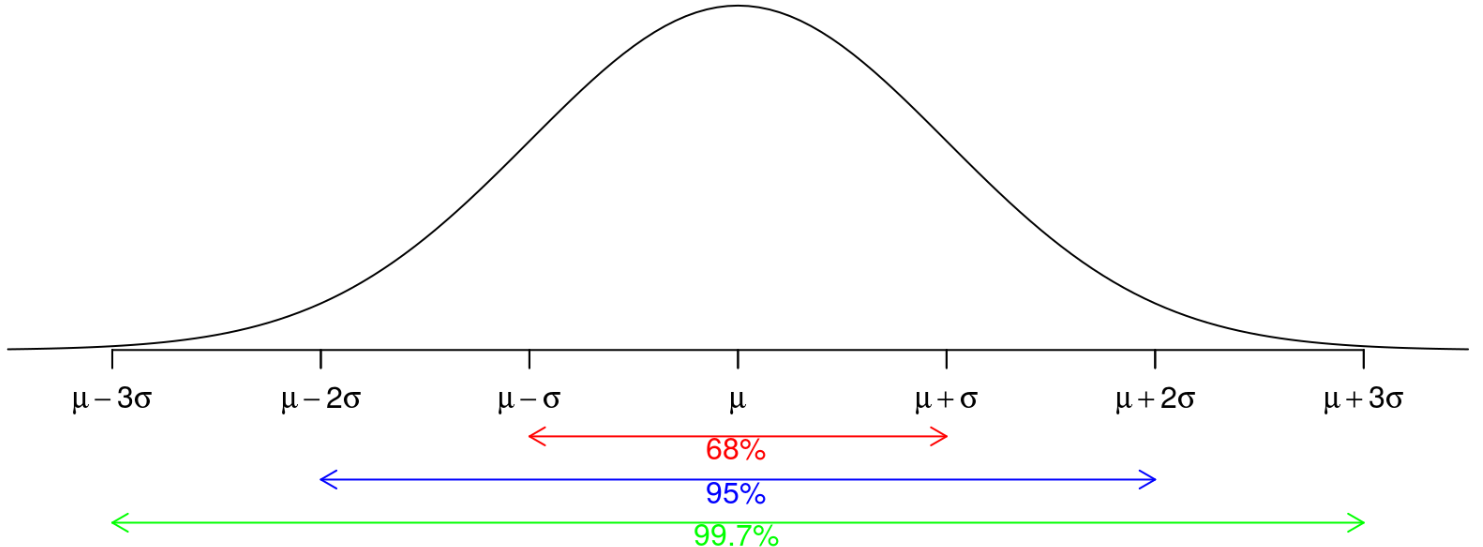
\includegraphics[width=0.75\linewidth]{images/Normalfordeling} 

}

\caption{Figurtekst}\label{fig:unnamed-chunk-2}
\end{figure}

Det gælder altså, at \(\approx 68 \%\) af observationerne findes inden for én standardafvigelse fra middelværdien, \(\approx 95 \%\) inden for to standardafvigelser og \(\approx 99,7 \%\) inden for tre standardafvigelser.

På baggrund af dette, kan en outlier defineres som en værdi, der ligger et vist antal standardafvigelser væk fra middelværdien. Som udgangspunkt siges det, at hvis en værdi er mere end \(3\) standardafvigelser væk fra middelværdien, kan den ses som en outlier.

En anden måde at beskrive fordelingen af en observation er ved hjælp af percentiler - et punkt for hvilket en hvis mængde af data antager værdier, der ligger over eller under punktet. Her en medianen et specialtilfælde af en percentil, 50-percentilen, hvor halvdelen af data antager værdier under punktet, og den anden halvdel over punktet. Generelt defineres en percentil som,

\begin{quote}
\BeginKnitrBlock{definition}
\protect\hypertarget{def:unnamed-chunk-3}{}{\label{def:unnamed-chunk-3} }\textbf{p-percentilen} er et punkt, således at \(p \%\) af observationerne antager værdier under punktet, og \((100 - p) \%\) af observationerne antager værdier over punktet.
\EndKnitrBlock{definition}
\end{quote}

To andre særlige tilfælde af percentiler er 25-percentilen, den nedre kvartil (\(Q_L\)), og 75-percentilen, den øvre kvartil (\(Q_U\)). Ved hjælp af \(Q_L\) og \(Q_U\) kan variabiliteten af observationerne beskrives som afstanden mellem de to kvartiler. Denne afstand benævnes \emph{Inner Quartile Range} (\emph{IQR}), og beregnes som \(IQR = Q_U - Q_L\).

Når både minimum, nedre kvartil, median, øvre kvartil og maksimum er fundet, kan disse benyttes til at tegne et boksplot af observationerne. Et boksplot giver et grafisk overblik af midten og variabiliteten af observationerne. Et boksplot ser ud, som på figuren nedenfor.

\begin{figure}

{\centering 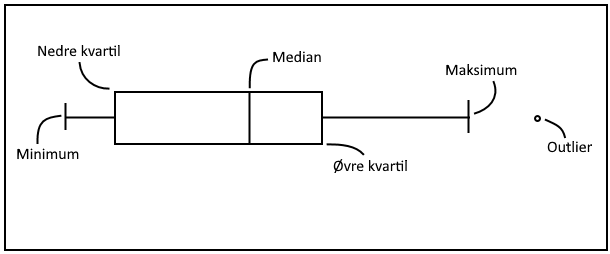
\includegraphics[width=0.75\linewidth]{images/Boksplot} 

}

\caption{Figurtekst}\label{fig:unnamed-chunk-4}
\end{figure}

På baggrund af \emph{IQR} og boksplottet kan outliers nu defineres som data, der antager værdier mere end \(1,5(IQR)\) gange over \(Q_U\) eller under \(Q_L\).

Outliers er altså værdier, der er ekstreme nok til at påvirke en dataanalyse i forkert retning. Derfor benyttes forskellige metoder til at identificere sådanne outliers, som derefter kan fjernes i en rengøring af datasættet.

\hypertarget{problemformulering}{%
\section{Problemformulering}\label{problemformulering}}

\emph{Hvorvidt kan simulationsstudier bidrage til at højne kvaliteten af dataanalyser?}

\begin{enumerate}
\def\labelenumi{\arabic{enumi}.}
\item
  Hvilke faldgruber skal man være opmærksom på?
\item
  Hvordan simulerer man data?
\end{enumerate}

\begin{enumerate}
\def\labelenumi{\alph{enumi}.}
\tightlist
\item
  Hvordan sikrer man en høj kvalitet af simuleret data?
\end{enumerate}

\begin{enumerate}
\def\labelenumi{\arabic{enumi}.}
\setcounter{enumi}{2}
\item
  Hvad kan man inferere ud fra simuleret data?
\item
  Hvilke alternativer finder der til statistisk inferens? (Bootstrapping)
\end{enumerate}

\hypertarget{faldgruber-i-en-dataanalyse}{%
\chapter{Faldgruber i en dataanalyse}\label{faldgruber-i-en-dataanalyse}}

Der er flere forskellige forhold at tage hensyn til, inden en dataanalyse påbegyndes. Nogle eksempler på disse forhold gennemgåes i dette kapitel, herunder variabeltyper, estimatorens egenskaber, fordelinger og antallet af kovariater. Afsnittet er primært skrevet med inspiration fra \citep{ASTAbog} og \citep{ASTAkursus3}.

\hypertarget{variabeltyper-1}{%
\section{Variabeltyper}\label{variabeltyper-1}}

I dette afsnit gennemgåes\ldots{} fordi\ldots{}

Som nævnt i \textbf{AFSNITTET}, findes der forskellige typer af variable. Dette er en vigtig faktor at tage hensyn til, da det har indflydelse på, hvilke matematiske operationer, der kan udføres på variablen. Desuden har variabeltypen indflydelse på, hvilken type diagram de kan illustreres i. En kort opsummering af, hvilke operationer, der kan udføres på hvilke variable, ses på tabellen nedenfor.

\begin{longtable}[]{@{}llll@{}}
\caption{En oversigt over de forskellige variable, og hvilke typer af matematiske operationer, der kan udføres på dem.}\tabularnewline
\toprule
Kvalitative variable & Kvantitative variable & &\tabularnewline
\midrule
\endfirsthead
\toprule
Kvalitative variable & Kvantitative variable & &\tabularnewline
\midrule
\endhead
\textbf{Nominal} & \textbf{Ordinal} & \textbf{Interval} & \textbf{Ratio}\tabularnewline
Andel & Median & Middelværdi & Middelværdi\tabularnewline
Frekvens & Kvartiler & Standardafvigelse & Standardafvigelse\tabularnewline
\bottomrule
\end{longtable}

Generelt gælder det, at hvis en variabel tillader en bestemt operation, tillades samme operation på variabler, der står til højre i tabellen.

En anden væsentlig, omend ikke lige så matematisk faldgrube, er symboler. Der defineres nøjagtigt, hvad en parameter, et estimat og en estimator er, og de hver et specifikt symbol. Generelt gælder, at græske bogstaver definerer en parameter, det tilsvarende latinske bogstav et estimat, og et stort latinsk bogstav en estimator. I tabellen nedenfor er det opsummeret, hvad fire forskellige parametre er givet som, og hvad det tilsvarende er i stikprøven og estimatoren.

\begin{longtable}[]{@{}ccc@{}}
\caption{En oversigt over de forskellige symboler, som angiver henholdsvis en parameter, et estimat og en estimator.}\tabularnewline
\toprule
Population (Parametre) & Stikprøve (Estimater) & Estimatorer\tabularnewline
\midrule
\endfirsthead
\toprule
Population (Parametre) & Stikprøve (Estimater) & Estimatorer\tabularnewline
\midrule
\endhead
my & my\_hat & My\_hat\tabularnewline
sigma & s & S\tabularnewline
sigma\^{}2 & s\^{}2 & S\^{}2\tabularnewline
pi & pi\_hat & Pi\_hat\tabularnewline
\bottomrule
\end{longtable}

Det er derfor klart, at der skal være enighed om, hvad en parameter og et estimat er, og hvad forskellen er på et estimat og en estimator, før en dataanalyse kan udføres korrekt.

\hypertarget{estimatorens-egenskaber}{%
\section{Estimatorens egenskaber}\label{estimatorens-egenskaber}}

I dette afsnit gennemgåes de forskellige egenskaber, unbiased, efficient, konsistent og sufficient, en estimator kan have. Disse begreber giver et indblik i, hvor god en estimator er, og derved også, hvor valide resultater, en dataanalyse på baggrund af den estimator, vil bibringe.

En estimator er en stikprøvefunktion, der udfører en beregning på baggrund af værdier i en stikprøve, for at estimere parametrene i en population. Eksempelvis er middelværdi, \(mean = \frac{\sum observationer}{\# observationer}\), en estimator, der beregner et estimat for en populations middelværdi.

Der findes overordnet set fire forskellige måder at måle, hvorvidt en estimator er passende for ens data. Disse er, om estimatoren er forventningsret, efficient, konsistent og sufficient, som defineret nedenfor.

\begin{quote}
\BeginKnitrBlock{definition}
\protect\hypertarget{def:unnamed-chunk-5}{}{\label{def:unnamed-chunk-5} }\textbf{Estimatorers egenskaber} \citep{ASTAkursus3}

\emph{Forventningsret}: Den forventede værdi for en forventningsret estimator er lig parameteren \(E(\hat{Y}) = \mu\).

\emph{Efficient}: En efficient estimator er den estimator med lavest varians.

\emph{Konsistent}: Variansen af en konsistent estimator falder, når størrelsen af stikprøven stiger.

\emph{Sufficient}: For en sufficient estimator gælder det, at når estimatet er beregnet, skal stikprøven ikke indeholde yderligere informationer om parameteret.
\EndKnitrBlock{definition}
\end{quote}

Hver af disse egenskaber har indvirkning på, hvor brugbare resultater, en dataanalyse vil bibringe. En estimator, der ikke er forventningsret, vil ikke give et korrekt bud på populationens middelværdi. Ligeledes vil en estimator, der ikke er efficient, have en større varians end mindst en anden estimator, hvilket leder til mindre brugbare resultater. Det er derfor vigtigt, at en estimator undersøges grundigt, og dens egenskaber bestemmes, inden den tages i brug.

\hypertarget{populationens-fordeling}{%
\section{Populationens fordeling}\label{populationens-fordeling}}

I dette afsnit gennemgåes, hvilken indflydelse en populations fordeling har på fordelingen af estimaterne og de tilhørende estimatorer. Dette er nødvendigt, da forskellige regneregler og metoder, der gælder for eksempelvis en normalfordeling ikke nødvendigvis gælder for eksempelvis en uniform fordeling.

\begin{itemize}
\tightlist
\item
  Population højreskæv -\textgreater{} estimat højreskæv og estimator højreskæv
\item
  Generel foldningsregel
\item
  Den centrale grænseværdisætning
\end{itemize}

\begin{quote}
\BeginKnitrBlock{theorem}
\protect\hypertarget{thm:unnamed-chunk-6}{}{\label{thm:unnamed-chunk-6} }\textbf{Den Centrale Grænseværdisætning} \citep[s. 93]{ASTAbog}.

Ved tilfældig stikprøveudtagning af tilpas stor størrelse, vil fordelingen af stikprøvegennemsnittet blive tilnærmelsesvist normalfordelt.
\EndKnitrBlock{theorem}
\end{quote}

\hypertarget{hvad-er-kovariater}{%
\chapter{Hvad er kovariater}\label{hvad-er-kovariater}}

Kovariater er variabler som beskriver responsvariablen. Responsvariablen er den variabel der ændre sig i forhold til de forklarende variabler (kovariater). Hvis man for eksempel vil lave en analyse af mænd og kvinders indkomst på arbejdsmarkedet, vil det give mening at tilføje en variabel der måler på arbejdserfaring, da den vil kunne antages at have en indflydelse på indkomsten. Kontrolvariablen der tilføjes som måler arbejdserfaring kaldes for en kovariat. Denne type sammenligning er kaldet ``analysis of covariance''. Hvis der ikke blev taget højde for, den ekstra variabel, arbejdserfaring og dermed kun ses på forholdet mellem indkomst og køn, ville den type sammenligning være ``analysis of variance''.

\hypertarget{hvorfor-og-hvordan-bruges-det}{%
\section{Hvorfor og hvordan bruges det}\label{hvorfor-og-hvordan-bruges-det}}

Fordi at indflydelse kan ændre sig efter at der kontrolleres for variabler (kovariater), kan resultaterne for ``analysis of covariance'' og ``analysis of variance'' være forskellige. For eksempel med indkomsten mellem mænd og kvinder, kan det siges at mere arbejdserfaring har positiv indflydelse på indkomsten. Hvis mænd tenderer til at have mere arbejdserfaring end kvinder, vil resultatet ændre sig, afhængig af om man kontroller for variablen arbejdserfaring. {[}ASTA-bogen{]}
Det kan dermed siges at kovariater er vigtige at tage højde for, da konklusionen af data afhænger af at der er blevet taget højde for alle kovariater der forklarer responsvariablen. Hvis man ikke har alle kovariater med, kan man komme til at konkluderer en forkert hypotese.

\hypertarget{simulering-af-variabler}{%
\chapter{Simulering af variabler}\label{simulering-af-variabler}}

Simuleringer er generering af estimater på mulige udfald, og på den måde efterligne virkeligheden ved simulering. Formålet er derved, at generere tilfældigt estimerede værdier ud fra en model, der simulerer virkeligheden, hvilket muliggører yderligerer analyser.

En defination på simulation er;

\begin{quote}
A situation or event that seems real but is not real, used especially in order to help people deal with such situations or events. - Cambridge Dictonary {[}\url{https://dictionary.cambridge.org/dictionary/english/simulation}{]}
\end{quote}

Ud fra definationen, er formålet altså ved simuleringer at efterligne virkeligheden, så de analyser der gøres på baggrund af simuleringerne, kan bruges i virkeligheden når lignende situationer opstår.
Brancher hvor simulationer er et yderst vigtigt redskab, er i motorsporten. I Formula 1, benytter holdene sig af simulatore, hvor de genskaber bilerne og derved kan teste nye dele af inden de behøver at producere dem i virkeligheden for at spare penge, så de derved kan analysere, hvad der for eksempel producere mere \emph{down-force} af forskellige dele, og så etablere den i stedet for, at skulle teste dem i virkeligheden. {[}\url{https://careers.mercedesamgf1.com/facilities/simulator/}{]}

\hypertarget{simulering-i-r}{%
\section{Simulering i R}\label{simulering-i-r}}

Simuleringer i R gøres ved at estimere udfald fra en fordeling, hvor der bliver genereret ``tilfældige'' tal. Eftersom tilfældige tal står i citationstegn, er det fordi, at der refereres til pseudo-tilfældige tal.
Disse generede tal forekommer at være tilfældige, men er det reelt set ikke helt tilfældige. {[}\url{https://en.wikipedia.org/wiki/Pseudorandom_number_generator}{]}

Tallene er genereret ud fra et \emph{seed}, som i R bestemmes ved set.seed(``værdi''). Generere man tal ud fra samme \emph{seed}, så vil værdierne altså være identiske.

Fordelinger som der blandt andet kan simuleres i R er normalfordelinger, binomialfordelinger og uniformefordelinger.

En normalfordeling kan simuleres på følgende måde:

\begin{Shaded}
\begin{Highlighting}[]
\KeywordTok{set.seed}\NormalTok{(}\DecValTok{1}\NormalTok{)}
\KeywordTok{rnorm}\NormalTok{(}\DecValTok{10}\NormalTok{, }\DataTypeTok{mean =} \DecValTok{0}\NormalTok{, }\DataTypeTok{sd =} \DecValTok{1}\NormalTok{)}
\end{Highlighting}
\end{Shaded}

\begin{verbatim}
##  [1] -0.6264538  0.1836433 -0.8356286  1.5952808  0.3295078 -0.8204684
##  [7]  0.4874291  0.7383247  0.5757814 -0.3053884
\end{verbatim}

Først sættes et \emph{seed}, så man kan rekonstruere samme simulation igen. Næste linje startes med at skrive ``rnorm'' hvor ``r'' står for tilfældigt genererede tal, og ``norm'' for en normalfordeling. Inde i parantesene angives antallet af værdier der skal genereres, som bliver genereret ud fra en middelværdi på 0 og en standardafvigelse på 1. Eftersom middelværdien er 0 og standardafvigelsen er 1, kaldes denne normalfordeling for en standard normalfordeling eller Z-fordeling.

Ligeledes kan man simulere binomialfordelinger og uniformefordelinger:

\begin{Shaded}
\begin{Highlighting}[]
\KeywordTok{set.seed}\NormalTok{(}\DecValTok{1}\NormalTok{)}
\KeywordTok{rbinom}\NormalTok{(}\DecValTok{10}\NormalTok{, }\DataTypeTok{size =} \DecValTok{2}\NormalTok{, }\DataTypeTok{prob =} \FloatTok{0.5}\NormalTok{)}
\end{Highlighting}
\end{Shaded}

\begin{verbatim}
##  [1] 1 1 1 2 0 2 2 1 1 0
\end{verbatim}

Som før sættes et \emph{seed}, og der skrives ``r'' før fordelingen der simuleres. Ligeledes er første værdi antallet af værdier der skal genereres. I binomialfordelingen er der angivet \emph{size}, som er antallet success/faliure \emph{(1/0)} repetationer, hvor hvor \emph{prob} er sandsynligheden for success.

\begin{Shaded}
\begin{Highlighting}[]
\KeywordTok{set.seed}\NormalTok{(}\DecValTok{1}\NormalTok{)}
\KeywordTok{runif}\NormalTok{(}\DecValTok{10}\NormalTok{, }\DataTypeTok{min =} \DecValTok{1}\NormalTok{, }\DataTypeTok{max =} \DecValTok{2}\NormalTok{)}
\end{Highlighting}
\end{Shaded}

\begin{verbatim}
##  [1] 1.265509 1.372124 1.572853 1.908208 1.201682 1.898390 1.944675 1.660798
##  [9] 1.629114 1.061786
\end{verbatim}

Uniformfordelingen er derimod angivet med en minimum og maximum-værdi, hvor der genereres værdier imellem.

\hypertarget{sample-og-replicate-bootstrapping}{%
\subsection{Sample og replicate (Bootstrapping)}\label{sample-og-replicate-bootstrapping}}

Derudover kan der simuleres på baggrund af observeret data. Ved at benytte \emph{sample} og \emph{replicate} fuktionerne kan der dannes nye simulationer. \emph{Sample} tager en stikprøve af den observerede data, hvor \emph{replicate} kan gentage forskellige stikprøver.

\begin{Shaded}
\begin{Highlighting}[]
\KeywordTok{set.seed}\NormalTok{(}\DecValTok{1}\NormalTok{)}
\NormalTok{Z_fordeling <-}\StringTok{ }\KeywordTok{rnorm}\NormalTok{(}\DecValTok{1000}\NormalTok{, }\DataTypeTok{mean =} \DecValTok{0}\NormalTok{, }\DataTypeTok{sd =} \DecValTok{1}\NormalTok{)}

\KeywordTok{mean}\NormalTok{(Z_fordeling)}
\end{Highlighting}
\end{Shaded}

\begin{verbatim}
## [1] -0.01164814
\end{verbatim}

Her eksekveres en Z-fordling af 1000 observationer hvor middelværdien, -0.01164814, printes. Denne middelværdi vil varriere afhængigt af det \emph{seed} der benyttes.

Dernæst kan der foretages en sample af Z\_fordeling.

\begin{Shaded}
\begin{Highlighting}[]
\KeywordTok{set.seed}\NormalTok{(}\DecValTok{1}\NormalTok{)}
\NormalTok{Z_sample <-}\StringTok{ }\KeywordTok{sample}\NormalTok{(Z_fordeling, }\DataTypeTok{size =} \DecValTok{10}\NormalTok{, }\DataTypeTok{replace =} \OtherTok{TRUE}\NormalTok{)}

\NormalTok{Z_sample}
\end{Highlighting}
\end{Shaded}

\begin{verbatim}
##  [1]  1.1654620  0.2109073 -0.6816605  0.3439100  1.1594245 -0.8132443
##  [7] -0.0505657 -0.9398293  0.5050676  1.4645873
\end{verbatim}

\begin{Shaded}
\begin{Highlighting}[]
\KeywordTok{mean}\NormalTok{(Z_sample)}
\end{Highlighting}
\end{Shaded}

\begin{verbatim}
## [1] 0.2364059
\end{verbatim}

Her fremgår der 10 værdier, som er taget fra Z\_fordeling, som gemmes i Z\_sample. \emph{Replace} gør så de værdier der tages og gemmes i Z\_sample bliver lagt tilbage, og kan derved blive taget igen, så man kan få den samme værdi flere gange.

Derefter er det muligt at gentage disse stikprøver ved brug af \emph{replicate}

\begin{Shaded}
\begin{Highlighting}[]
\KeywordTok{set.seed}\NormalTok{(}\DecValTok{1}\NormalTok{)}
\NormalTok{Z_replicate <-}\StringTok{ }\KeywordTok{replicate}\NormalTok{(}\DecValTok{100}\NormalTok{, \{}
\NormalTok{  x <-}\StringTok{ }\KeywordTok{mean}\NormalTok{(}\KeywordTok{sample}\NormalTok{(Z_fordeling, }\DataTypeTok{size =} \DecValTok{10}\NormalTok{, }\DataTypeTok{replace =} \OtherTok{TRUE}\NormalTok{))}
\NormalTok{\})}
\NormalTok{Z_replicate}
\end{Highlighting}
\end{Shaded}

\begin{verbatim}
##   [1]  0.025838777 -0.203406868 -0.018837976  0.124819713 -0.164830739
##   [6]  0.333733810 -0.423105712 -0.184935071  0.032046950 -0.166711138
##  [11]  0.128328946 -0.003149890  0.120181675  0.114612739  0.196252732
##  [16] -0.503558064 -0.057580606  0.448834352  0.302573714  0.349289426
##  [21]  0.042763308 -0.449645007 -0.567764002 -0.246353993  0.241230288
##  [26]  0.118362694  0.360972297 -0.502740430 -0.294227992  0.116454913
##  [31] -0.458241385  0.145491729  0.468018395 -0.336889894 -0.033331555
##  [36]  0.003202705 -0.230521260  0.002509074 -0.104908678  0.577232470
##  [41]  0.405361935  0.571805412 -0.242967988 -0.070361799 -0.204749550
##  [46]  0.529131107  0.123788480  0.428641140  0.421487366  0.296227471
##  [51] -0.021464536 -0.563489156 -0.096866861  0.011460957  0.490675566
##  [56]  0.118853950 -0.048831160 -0.433364372 -0.158288527  0.228563345
##  [61]  0.383487805 -0.348257409  0.251253782  0.071396170  0.263839481
##  [66] -0.659980071 -0.272080635 -0.065224329  0.133837717 -0.278633082
##  [71] -0.543857905  0.066031905  0.675680619  0.172629193 -0.132092862
##  [76]  0.269779598  0.150154779 -0.214823863 -0.098373108 -0.102126967
##  [81] -0.350372760  0.502067558  0.111435486 -0.269840347  0.159325611
##  [86]  0.033092712 -0.180166957  0.284144813 -0.108679711  0.028228077
##  [91] -0.375649589 -0.224793309 -0.128662553  0.074568112  0.052000689
##  [96] -0.061919916  0.245951870  0.073717038 -0.297133939  0.034445758
\end{verbatim}

\begin{Shaded}
\begin{Highlighting}[]
\KeywordTok{mean}\NormalTok{(Z_replicate)}
\end{Highlighting}
\end{Shaded}

\begin{verbatim}
## [1] 0.004120227
\end{verbatim}

Her bliver en stikprøve af Z\_fordeling foretage 10x100 gange, hvorefter middelværdien på de 100 gentagelser bliver fundet.

Det med at tage en et stort antal stikprøver af nogle observationer er også kaldet bootstrapping, hvilket forklares i {[}AFSNIT XXXX{]}

Henvises der ikke til noget er kilden: {[}\url{https://bookdown.org/rdpeng/rprogdatascience/simulation.html}{]}
\textbf{AFSNIT SLUT}

\hypertarget{simulering-af-nominele-variabler}{%
\subsection{Simulering af nominele variabler}\label{simulering-af-nominele-variabler}}

En nominel variabel kan for eksempel være køn, en måde at simulere dette på kan være ved en binomialfordeling.

\begin{Shaded}
\begin{Highlighting}[]
\KeywordTok{set.seed}\NormalTok{(}\DecValTok{1}\NormalTok{)}
\NormalTok{gender <-}\StringTok{ }\KeywordTok{rbinom}\NormalTok{(}\DecValTok{100}\NormalTok{, }\DataTypeTok{size =} \DecValTok{1}\NormalTok{, }\DataTypeTok{prob =} \FloatTok{0.5}\NormalTok{)}
\KeywordTok{mean}\NormalTok{(gender)}
\end{Highlighting}
\end{Shaded}

\begin{verbatim}
## [1] 0.48
\end{verbatim}

Hvis kvinde er en success og mand er en failiure, så er der derved en forekomst på 48\% kvinder og 52\% mænd. Derved har binomialfordelingen taget 100 værdier, en gang, hvor der har været 50\% sandsynlighed for success, som har været kvinde. Da middelværdien er 0.48, betyder det så at der ud fra 100 observationer er 48 kvinder.

\hypertarget{simulering-af-ordinale-variabler}{%
\subsection{Simulering af ordinale variabler}\label{simulering-af-ordinale-variabler}}

En ordinal variabel, som der kan simuleres kan være minutter det tager at løse en opgave, hvilket kan simuleres ved en uniformfordeling.

\begin{Shaded}
\begin{Highlighting}[]
\KeywordTok{library}\NormalTok{(mosaic)}
\end{Highlighting}
\end{Shaded}

\begin{Shaded}
\begin{Highlighting}[]
\KeywordTok{set.seed}\NormalTok{(}\DecValTok{1}\NormalTok{)}
\NormalTok{opgave <-}\StringTok{ }\KeywordTok{as.integer}\NormalTok{(}\KeywordTok{runif}\NormalTok{(}\DecValTok{100}\NormalTok{, }\DataTypeTok{min =} \DecValTok{1}\NormalTok{, }\DataTypeTok{max =} \DecValTok{10}\OperatorTok{+}\DecValTok{1}\NormalTok{))}
\KeywordTok{gf_histogram}\NormalTok{(}\OperatorTok{~}\NormalTok{opgave, }\DataTypeTok{bins =} \DecValTok{10}\NormalTok{)}
\end{Highlighting}
\end{Shaded}

\includegraphics{bookdown-demo_files/figure-latex/unnamed-chunk-15-1.pdf}

\hypertarget{simulering-af-interval-variabler}{%
\subsection{Simulering af interval variabler}\label{simulering-af-interval-variabler}}

En interval variabel kan for eksempel simuleres ved

\hypertarget{simulering-af-ratio-variabler}{%
\subsection{Simulering af ratio variabler}\label{simulering-af-ratio-variabler}}

``\ldots{}''

Test

\emph{Magnus}
\textbf{Kan man sige ting om en population ud fra stikprøver (inferens, hvordan og hvorfor?)}

Processen med at bruge data analyse til at sige noget om en underliggende population ud fra en stikprøve, kaldes også statistisk inferens. Ud fra denne stikprøve vil man lave statistike analyser, som man kan bruge til at fortælle om populationen. Dette er meget nyttig, da det kan være nemmere at indsamle og analysere data fra en mindre mængde og så sige noget om en større mængde, end hvis man skulle indsamle mange millioner datapunkter.

I statistisk inferens differentier man normalt imellem to metoder, estimering og hypotesetest.
Når man estimerer noget ud fra en population, vil man bruge stikprøven til at beskrive en ukendt del af populationen. Det kan f.ek.s være gennemsnitsindkomst af danskere, hvorved man finder et estimat \(\mu^\) som bruges til at beskrive \(\mu\). Dette vil være et punkt estimat, og vil oftest suppleres med at intervalestimat. Da punkt estimater i sin essesns er tilfældig (den vil ændre sig fra stikprøve til stikprøve), vil man helst undgå at støtte sig 100 procent op af dette når man skal konkludere noget om populationen, og derfor vil man helst have et interval at kunne henvise til. Her vil man finde det interval, hvor man er enten ca. 95\% sikker på at \(\mu\) ligger inden for.
Den anden form for statistisk inferenes, nemlig hypotesetest, bruges til at bestemme om en teori om befolkningen viser sig at være sand. Det kunne være at hypotesen er, at danskere tjener mere i gennemsnit end folk fra Sverige. Der vil også typisk opstilles en modsat hypotese, i tilfældet af at vores første hypotese, \(H_0\) viser sig at være falsk. Denne modsat hypotese vil oftest blot sige det modsatte og kaldes for \(H_A\).

Et alternativ til statistisk inferens er bootstrapping -\textgreater{} Overgang?

\bibliography{book.bib,packages.bib}

\end{document}
